%\documentclass{article}
%\usepackage[a4paper, total={6in, 8in}]{geometry}
%\documentclass[reprint,amsmath,amssymb,rmp,onecolumn,notitlepage,11pt]{revtex4-1}
\documentclass[notitlepage,
reprint,%twocolumn,
%preprint
onecolumn,
amsmath,amssymb,superscriptaddress,aps,
pre,floatfix]{revtex4-1}
\usepackage[utf8]{inputenc}
%\usepackage{authblk}
%\usepackage{natbib}
\usepackage[normalem]{ulem}
\usepackage{graphicx}
\usepackage{hyperref}
\usepackage{tabularx}
\usepackage{multirow}
\usepackage{algorithm}
\usepackage{algpseudocode}
\usepackage{xcolor}
\newcommand{\red}[1]{\textcolor{red!80!black}{#1}}
\newcommand{\blue}[1]{\textcolor{blue!80!black}{#1}}
\newcommand{\green}[1]{\textcolor{green!70!black}{#1}}
\newcommand{\gray}[1]{\textcolor{gray!80!black}{#1}}
\usepackage{mathtools}
\DeclarePairedDelimiter{\evdel}{\langle}{\rangle}
\usepackage[colorinlistoftodos]{todonotes}
\newcommand{\Pin}{P_{\mathrm{in}}}
\newcommand{\fhigh}{f_{\mathrm{high}}}
\newcommand{\flow}{f_{\mathrm{low}}}
\setlength {\marginparwidth }{2cm}


\begin{document}
\title{Supplemental material accompanying "What geometrically constrained protein models can tell us about real-world protein contact maps"}
\author{Nora Molkenthin}
\email[Author to whom correspondence should be addressed:]{nora.molkenthin@pik-potsdam.de}
\affiliation{Potsdam Institute for Climate Impact Research, Germany}
\author{J. Jasmin  Güven}
\affiliation{EaStCHEM School of Chemistry, University of Edinburgh, Edinburgh, United Kingdom}
\author{Steffen Mühle}
\affiliation{Max-Planck Institute for Dynamics and Self-Organization (MPIDS), Am Faßberg 17, 37077 Göttingen, Germany}
\author{Antonia S. J. S. Mey}
\email[Author to whom correspondence should be addressed:]{antonia.mey@ed.ac.uk}
\affiliation{EaStCHEM School of Chemistry, University of Edinburgh, Edinburgh, United Kingdom}
\maketitle

\section*{Pseudoalgorithms for creating protein contact maps from protein data}

Algorithm~\ref{alg:pcm} describes how we construct PCMs from structural pdb files. We loop through all files and find all C$_\alpha$ atoms from each structure to calculate the pairwise C$_\alpha$ distances. If the distance is less than 8~Å, a contact ($A_{ij}=1$) is recorded in the adjacency matrix. Similarly, Algorithm~\ref{alg:dist} describes how we compute the amino acid distances from amino acids who are in close contact.
 
\begin{algorithm}[htb]
\caption{Creating PCMs from pdb structure files}\label{alg:pcm}
\begin{algorithmic}[1]
\For{\texttt{structure} in \texttt{structure}}\Comment{Read each pdb file}
\For{C$_\alpha^{(i)}$ and C$_\alpha^{(j)}$ in \texttt{pdb}}\Comment{Get all C$_\alpha$}
\State Compute $d_{ij}=|d_i-d_j|$ \Comment{Distance in Å}
\If{$d_{ij}\leq 8\;$Å}
    \State \texttt{$A_{ij}=1$} \Comment{Contact}
\Else
    \State \texttt{$A_{ij}=0$} \Comment{No contact}
\EndIf
\EndFor
\EndFor
\end{algorithmic}
\end{algorithm}

\begin{algorithm}[htb]
\caption{Amino acid distances from PCMs}\label{alg:dist}
\begin{algorithmic}[1]
\For{i in $\mathbf{A}^{\mathrm{struc}}$}\Comment{Loop over rows}
\For{j in $\mathbf{A}^{\mathrm{struc}}$}\Comment{Loop over columns}
\If{$A_{ij}=1$} \Comment{If contact, get distance}
    \State s = $|i - j|$
\EndIf
\EndFor
\EndFor
\end{algorithmic}
\end{algorithm}

\section*{Amino acid distance distributions of other chain lengths}
\subsection{AlphaFold 2}
Fig.~\ref{fig:alphafold} shows the amino acid distance distributions for protein contact maps calculated from AlphaFold~2 data in the chain length ranges of $L \approx 100$ amino acids ($85 \leq L \leq 115$, light green circles), $L \approx 200$ amino acids ($185 \leq L \leq 215$, medium green squares) and $L \approx 300$ amino acids ($285 \leq L \leq 315$, dark green triangles). The plot shows the approximate power law behaviour of the distribution. 

\begin{figure*}[htb]
    \centering{
    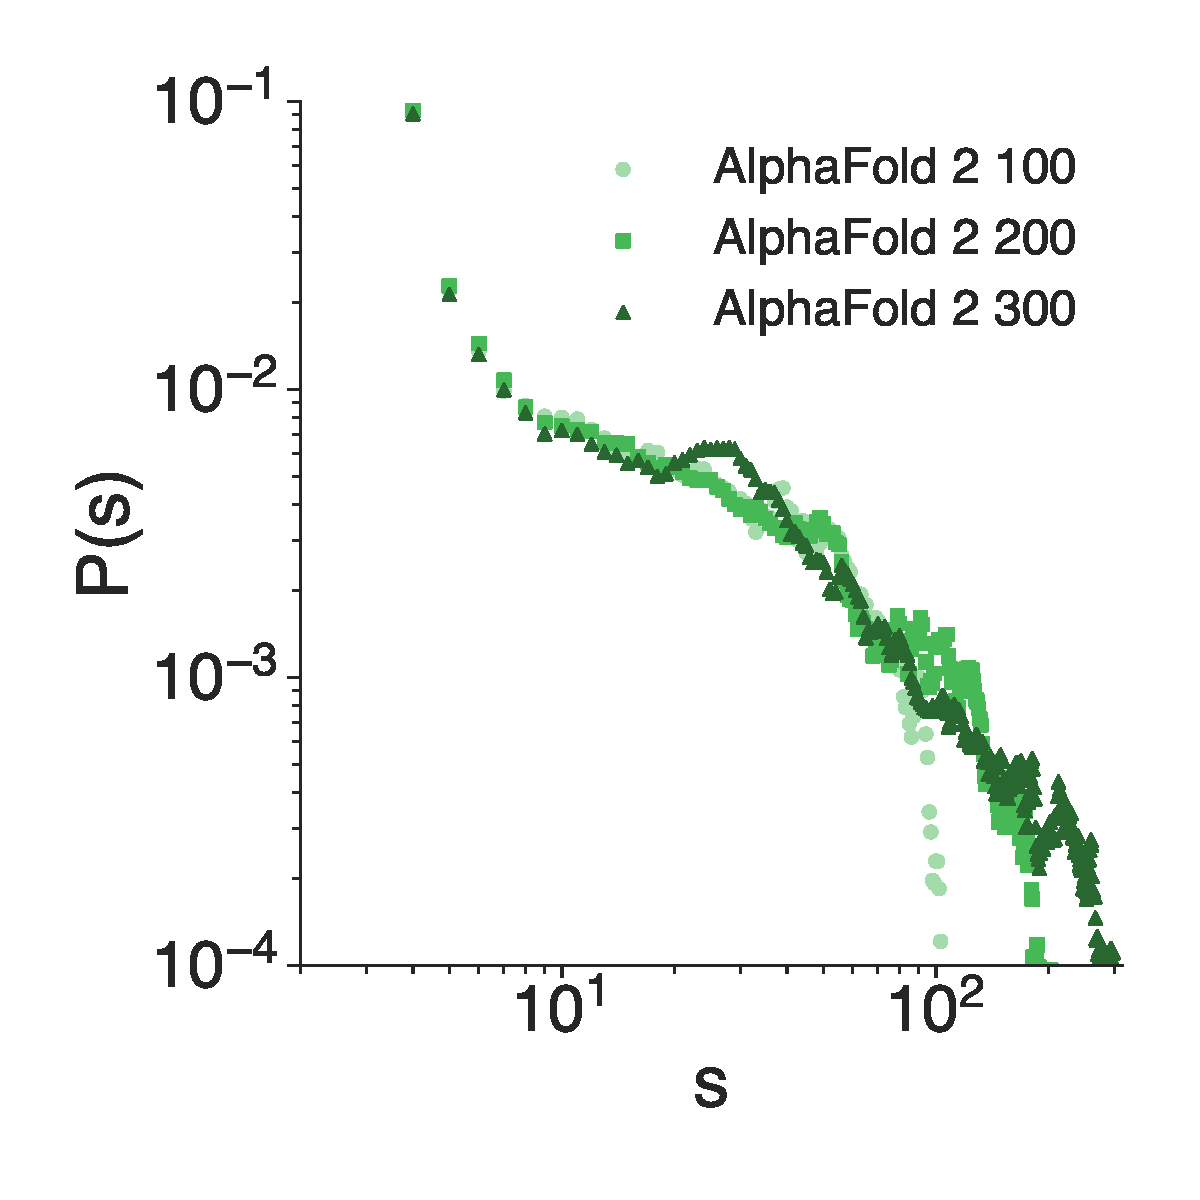
\includegraphics[width=\columnwidth]{paper/figures/SM_figures/alpha_chain_comparison.pdf}
    \caption{Amino acid distance distributions for contact maps derived from the AlphaFold 2 database for protein chains in the ranges of $L \approx 100$ amino acids ($85 \leq L \leq 115$, light green circles), $L \approx 200$ amino acids ($185 \leq L \leq 215$, medium green squares) and $L \approx 300$ amino acids ($285 \leq L \leq 315$, dark green triangles).}
    \label{fig:alphafold}}
\end{figure*}

\subsection{RCSB PDB and three-dimensional simulations}

Fig.~\ref{fig:rcsb_combined} a shows the amino acid distance distributions for protein contact maps calculated from structures in the chain length range $L\approx100$ amino acids for RCSB PDB (dark purple circles) and AlphaFold~2 (dark green squares). The shaded area shows the 95\% confidence level. Also shown are the analytic approximation and a general power law fitted to the RCSB data and their fit parameters, $a$ and $\Gamma$ for the analytical approximation and exponent $\gamma$ for the power law,  are shown in~Table~\ref{table:stats}. Similarly, Fig.~\ref{fig:rcsb_combined} shows the amino acid distance distributions for protein contact maps calculated from structures in the chain length range $L\approx200$ amino acids for RCSB PDB. We also computed the Kolmogorov-Smirnov (KS) statistic between the RCSB PDB and AlphaFold 2 distributions for each length range. The KS statistics were 0.07 and 0.10 for the ranges $L\approx100$ amino acids and $L\approx200$ amino acids, respectively. For both of these, the null hypothesis was accepted at the $\alpha=0.01$ level.

Fig.~\ref{fig:sim_3d} shows the amino acid distance distributions for protein contact maps calculated from the three-dimensional simulations. As before, the analytic approximation was fitted to the data in each range and the shaded area shows the 95\% confidence interval. The fit parameters $a$ and $\Gamma$ are given in Table~\ref{table:stats} for ranges $L\approx100$ amino acids,  $L\approx200$ amino acids and $L\approx300$ amino acids.

Finally, Fig.~\ref{fig:dc} shows the effect of changing the threshold value for determining contacts between amino acids for contact maps calculated from RCSB PDB, for a)  $L\approx100$ amino acids,  b) $L\approx200$ amino acids and c) $L\approx300$ amino acids.

% \begin{table}[tb]
% \centering
% \setlength{\tabcolsep}{10pt}
% \begin{tabular}{ c c c c}
% \hline
%  Data  & $\Gamma$ ($10^{-3}$) & $a$ & $\gamma$ \\
% \hline
%  RCSB 100 & 1.57 $\pm$ 0.51  & 2 $\pm$ 1 &  0.88 $\pm$ 0.02\\
%  RCSB 200 & 0.81 $\pm$ 0.19 & 2 $\pm$ 1 & 0.95 $\pm$ 0.02 \\
%  RCSB 300 & 0.74 $\pm$ 0.08 & 4 $\pm$ 1 & 1.45 $\pm$ 0.02 \\
%  3D SIM 100 & 3.1 $\pm$ 0.6 & 2 $\pm$ 1 & --  \\
%  3D SIM 200 & 1.2 $\pm$ 0.4 & 1 $\pm$ 1  & --  \\
%  3D SIM 300 & 7.0 $\pm$ 0.2 & 1 $\pm$ 1 & -- \\
%  2D SIM & 0.3 $\pm$ 0.1 & 6 $\pm$ 1 & -- \\
% \hline
% \end{tabular}
%  \caption{Parameters $a$ and $\Gamma$ for the analytical approximation, exponent $\gamma$ for the power law fit, and their uncertainties from fitting to amino acid distributions obtained from RCSB proteins in the chain length range $L\approx100$  and $L\approx200$ amino acids. Shown also are the fit parameters $a$ and $\Gamma$ from fitting the analytic approximation to the 3D simulations of chains in the $L\approx100$ and $L\approx200$ ranges.}
% \label{table:stats}
% \end{table}

\begin{table}[tb] 
\centering
\setlength{\tabcolsep}{10pt}
{\renewcommand{\arraystretch}{1.5}
\begin{tabular}{c c c c c c c c}
\hline
\multirow{2}{*}{Parameter}&\multicolumn{3}{c}{RCSB}& \multicolumn{3}{c}{3D Simulation}&\multirow{2}{*}{2D Simulation}
\\&100&200&300&100&200&300&\\
\hline
$\Gamma\; (10^{-3})$ & $1.57 \pm 0.51$ & $0.81 \pm 0.19 $ & $0.74 \pm 0.08$ & $3.1 \pm 0.6$ & $1.2 \pm 0.4$ & $7.0 \pm 0.2$ & $0.3 \pm 0.1$ \\
$a$ & $2 \pm 1$ & $2 \pm 1$ & $4 \pm 1$ & $2 \pm 1$ & $1 \pm 1$ & $1 \pm 1$ & $6 \pm 1$ \\
$\gamma$ & $0.88 \pm 0.02$ & $0.95 \pm 0.02$ & $1.45 \pm 0.02$ & - & - & - & - \\
 \hline
\end{tabular}
}
 \caption{Parameters $a$ and $\Gamma$ for the analytical approximation, exponent $\gamma$ for the power law fit, and their uncertainties from fitting to amino acid distributions obtained from RCSB PDB structures in ranges $L\approx100$ amino acids, $L\approx200$ amino acids and $L\approx300$ amino acids. Shown also are the fit parameters $a$ and $\Gamma$ from fitting the analytic approximation to the 2D simulation and 3D simulations of chains in the $L\approx100$, $L\approx200$ and $L\approx300$ ranges.}
\label{table:stats}
\end{table}




\begin{figure*}[htb]
    \centering{
    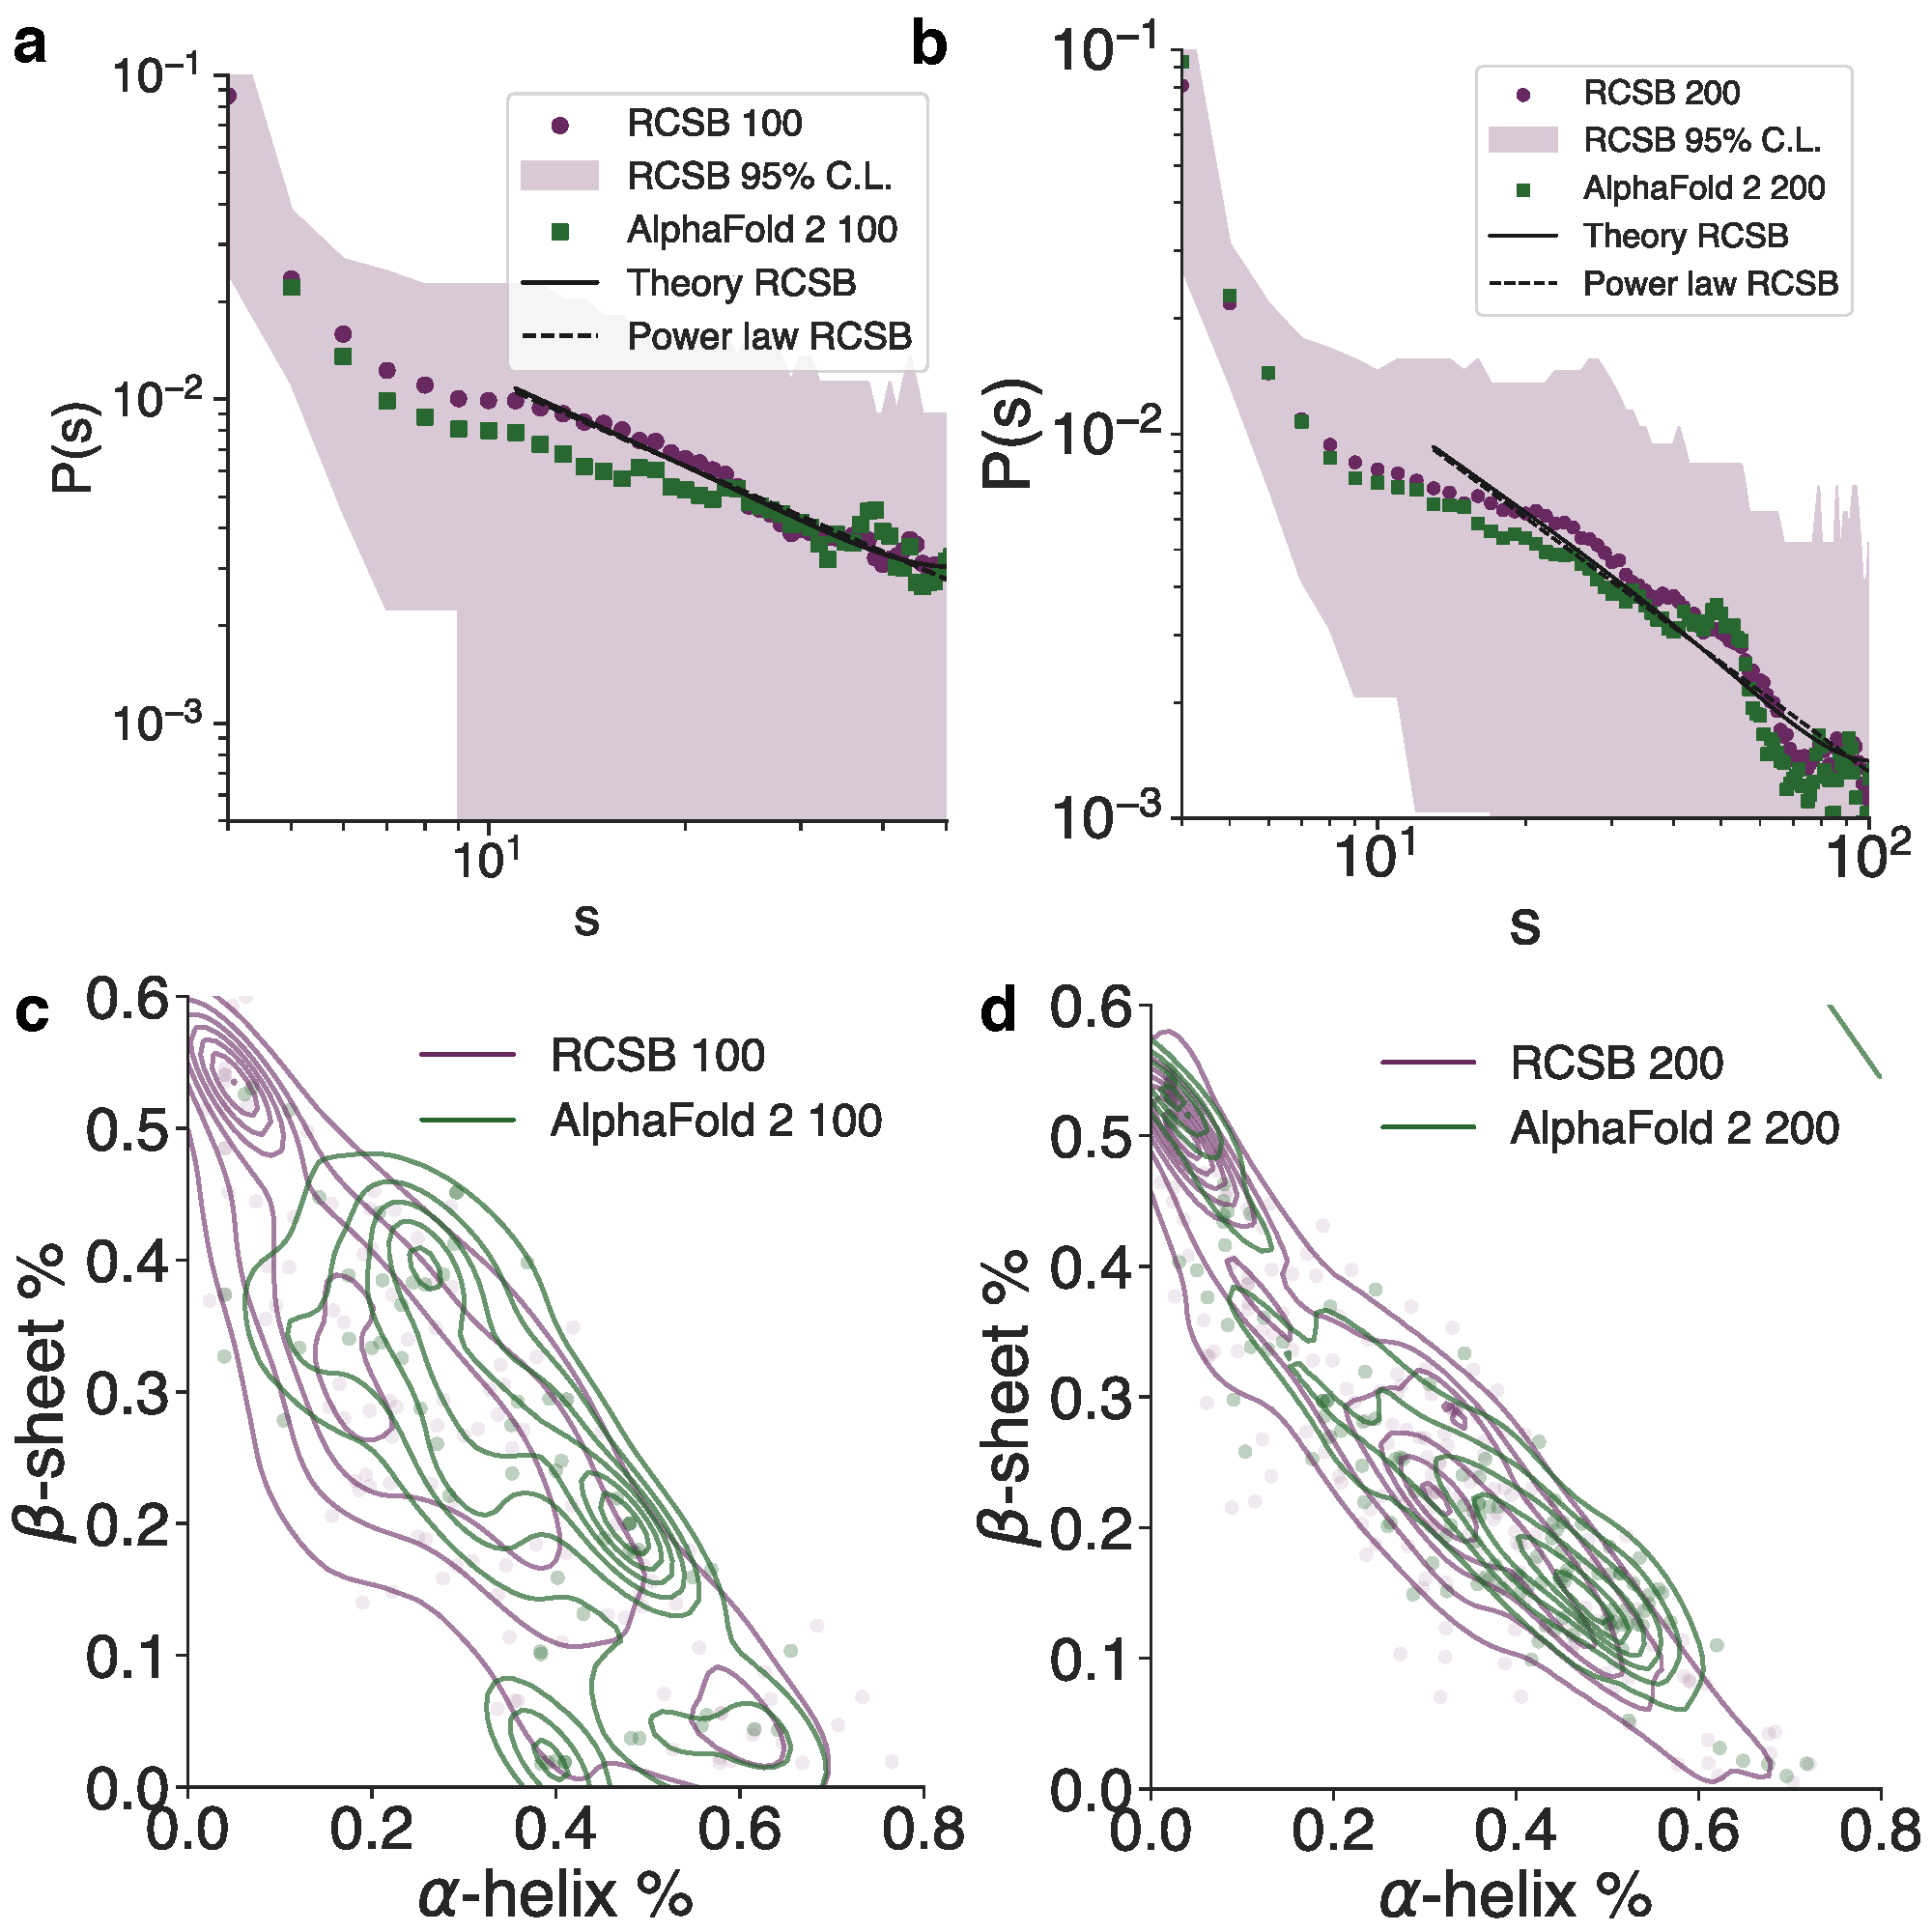
\includegraphics[width=\columnwidth]{paper/figures/SM_figures/distributions_combined.pdf}
    \caption{Comparison between the distributions of RCSB PDB and AlphaFold 2 database. The analytic approximation (solid line) and power law (dashed line) are fitted to the the RCSB PDB data. Pink shaded area shows the 95\% confidence level. The comparison is shown for two protein chain length ranges: a) $L\approx 100$ and b) $L\approx200$ range. Secondary structure content distribution in the RCSB and AlphaFold 2 structures in the  c) $L\approx100$ and the d) $L\approx200$ chain length range.}
    \label{fig:rcsb_combined}}
\end{figure*}

% \begin{figure*}[htb]
%     \centering{
%     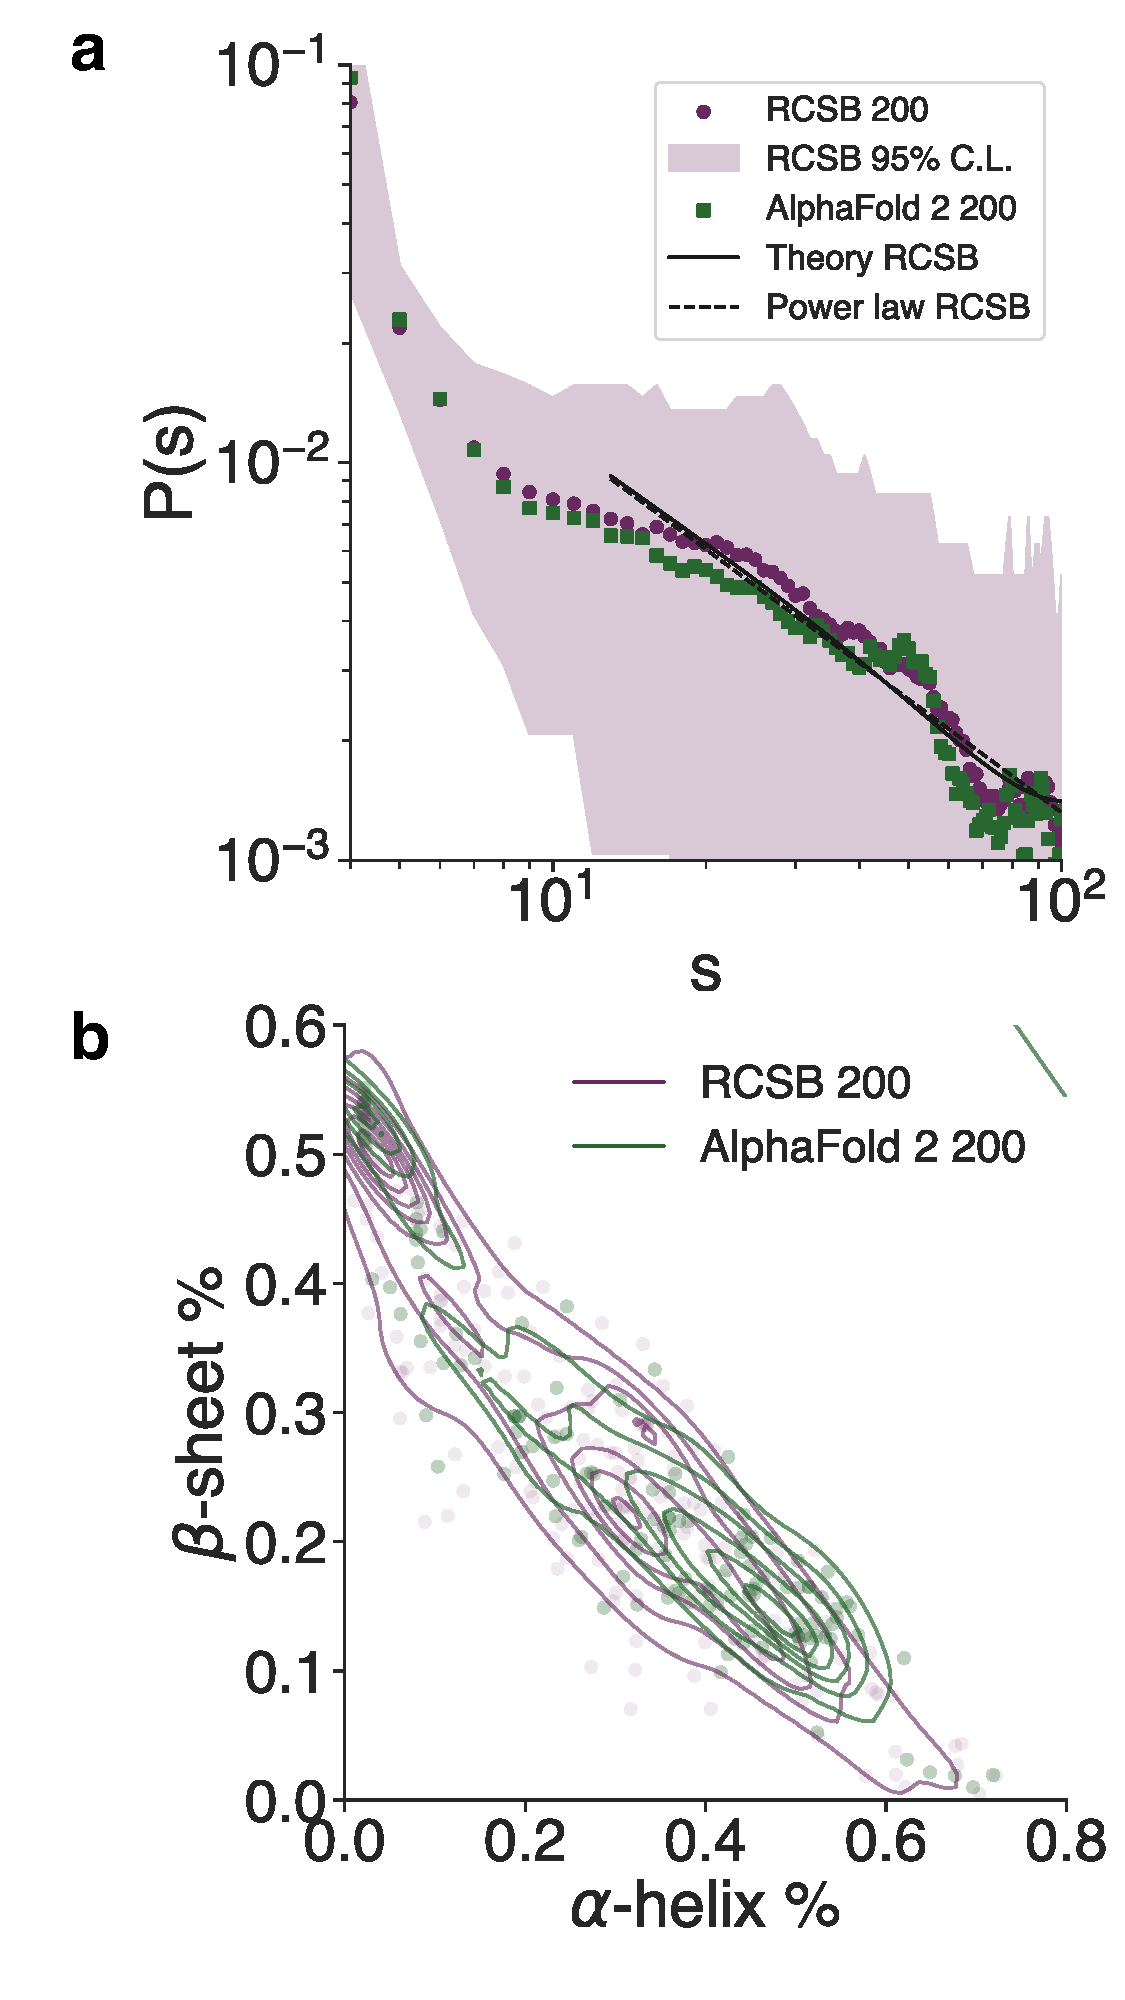
\includegraphics[scale=0.35]{paper/figures/SM_figures/distributions_200.pdf}
%     \caption{Comparison between the distributions of RCSB~\cite{PDB} and AlphaFold 2~\cite{jumper2021highly} databases for protein chains in the $L\approx200$ range. The analytic approximation (solid line) and power law (dashed line) are fitted to the tail of the RCSB data. Pink shaded area shows the 95\% confidence level.}
%     \label{fig:rcsb_200}}
% \end{figure*}

\begin{figure*}[htb]
    \centering{
    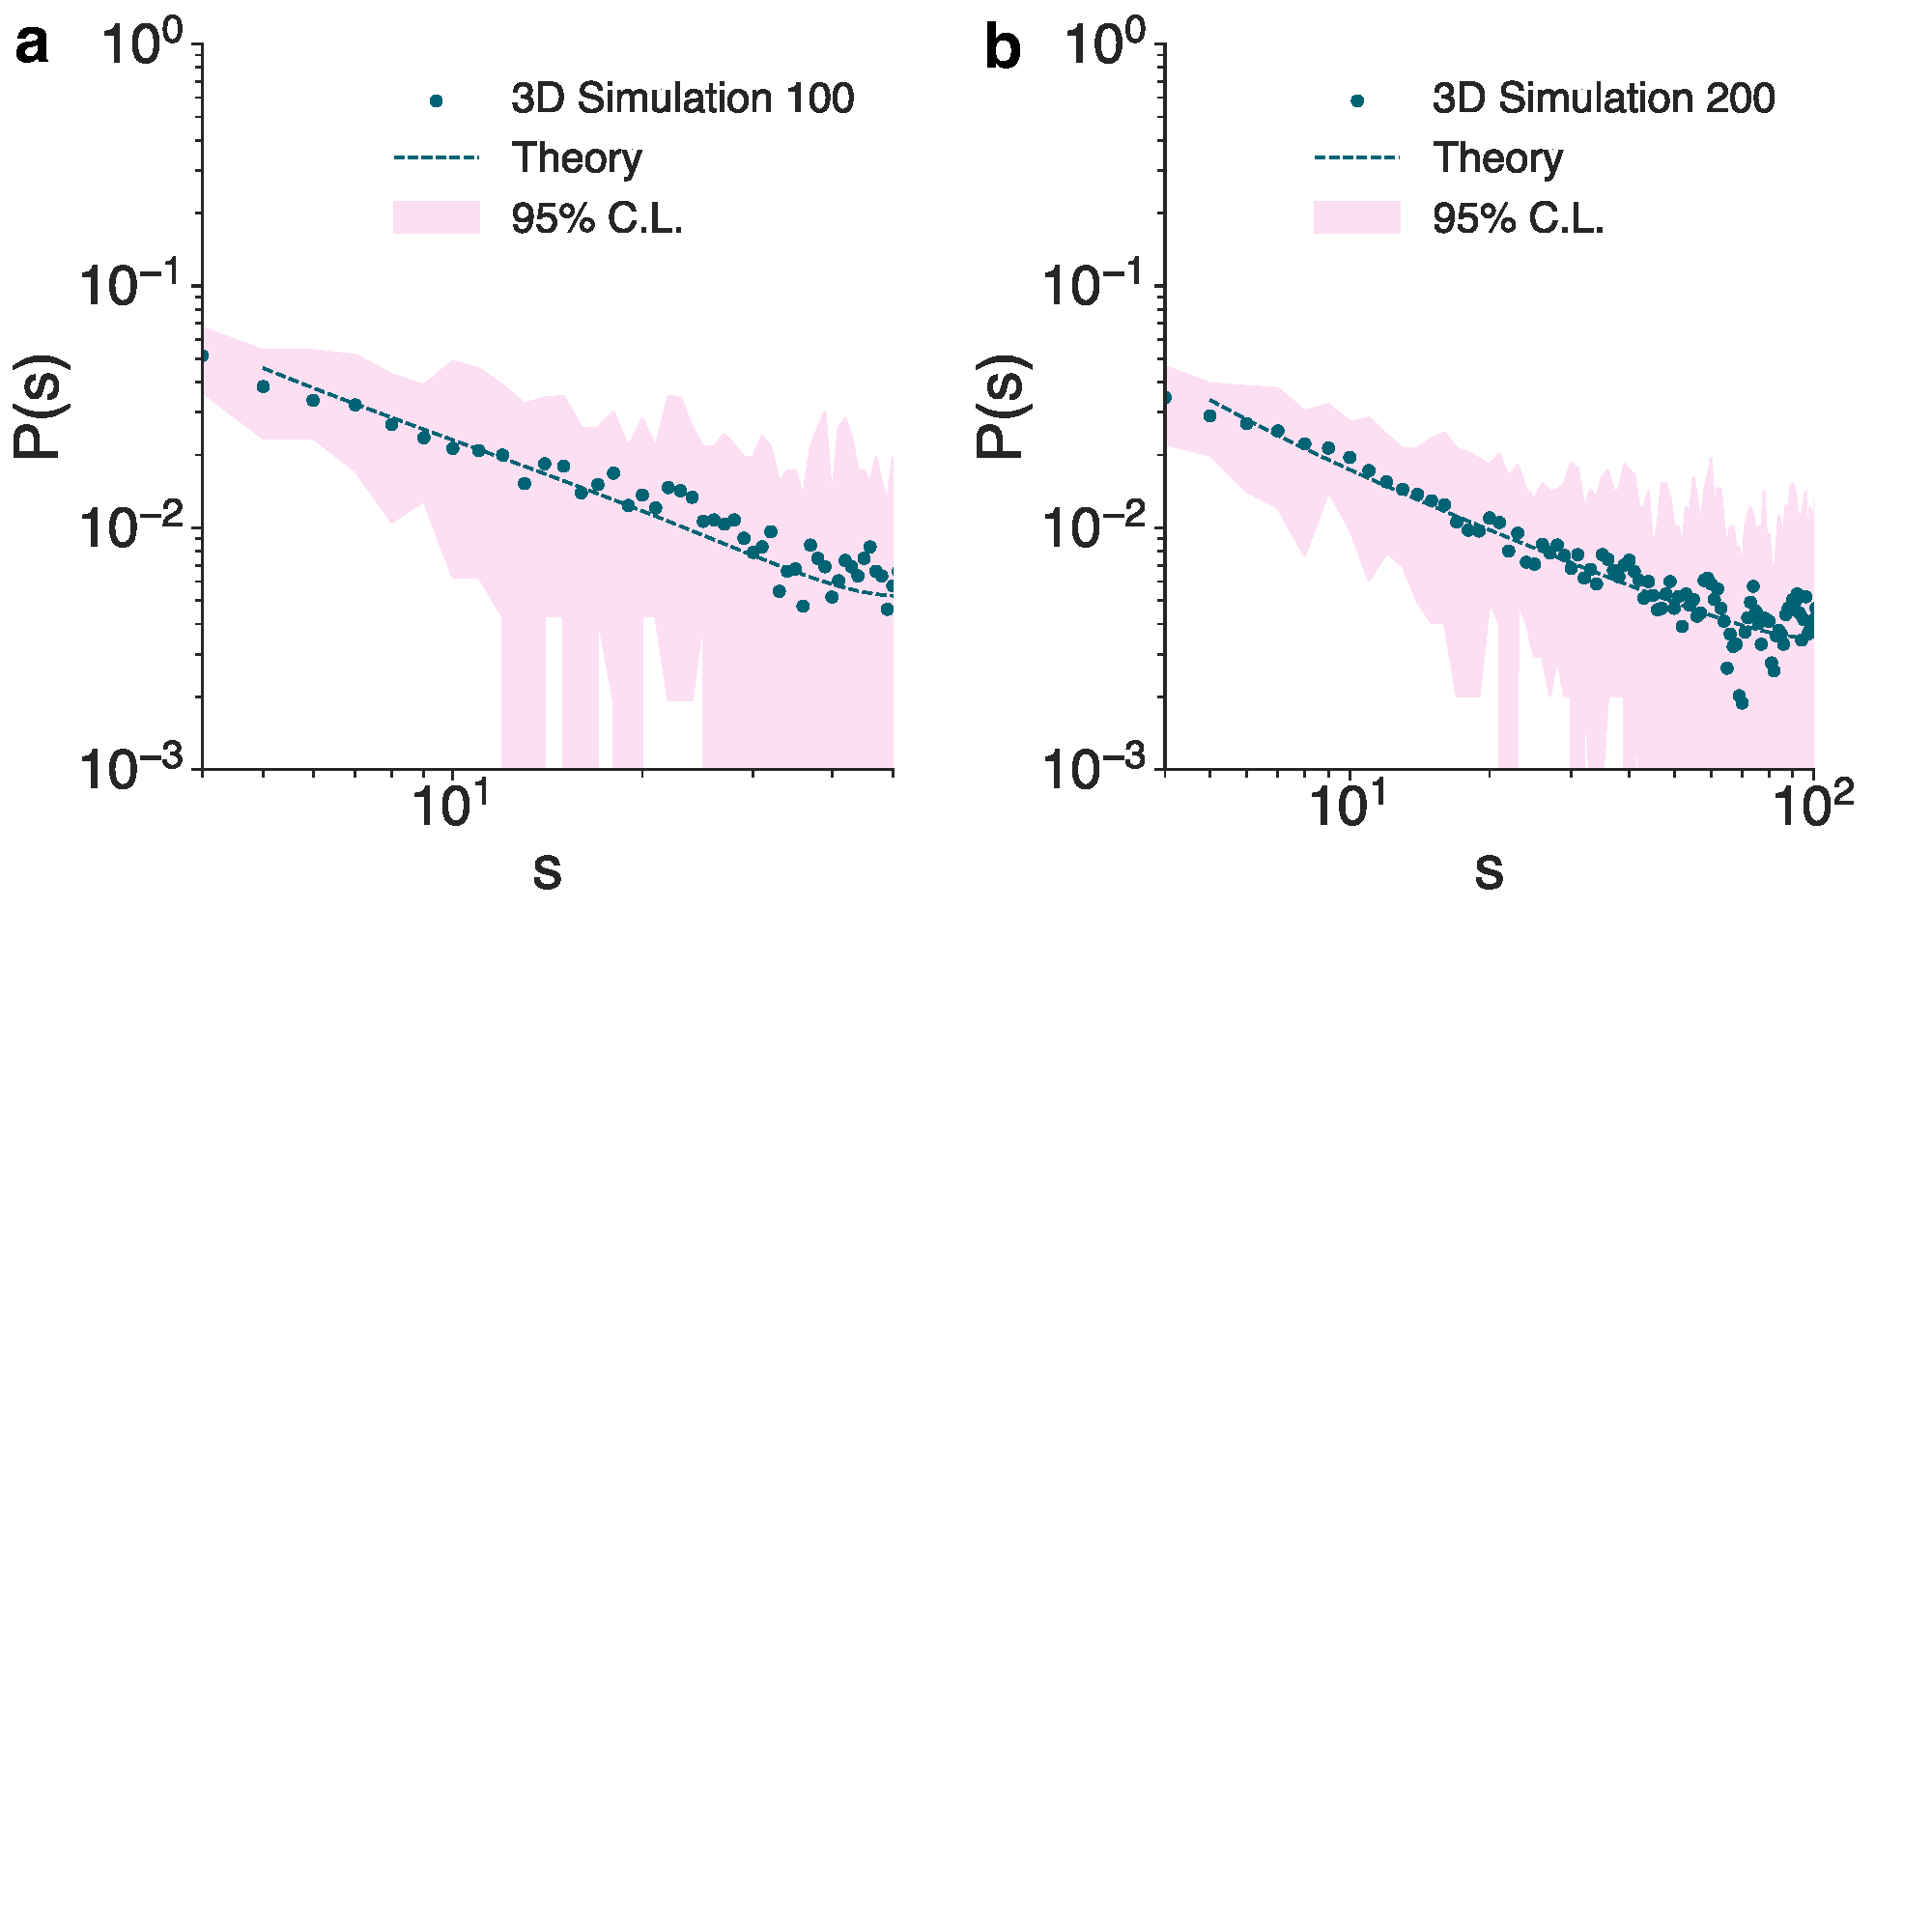
\includegraphics[width=\columnwidth]{paper/figures/SM_figures/simulations_3d.pdf}
    \caption{Amino acid distance distributions obtained from three-dimensional simulations for chains in the ranges a) $L\approx100$  and b) $\approx200$ amino acids. The dotted line shows the analytical approximation fitted to the data and the shaded area shows the 95\% confidence level.}
    \label{fig:sim_3d}}
\end{figure*}

\begin{figure*}[htb]
    \centering{
    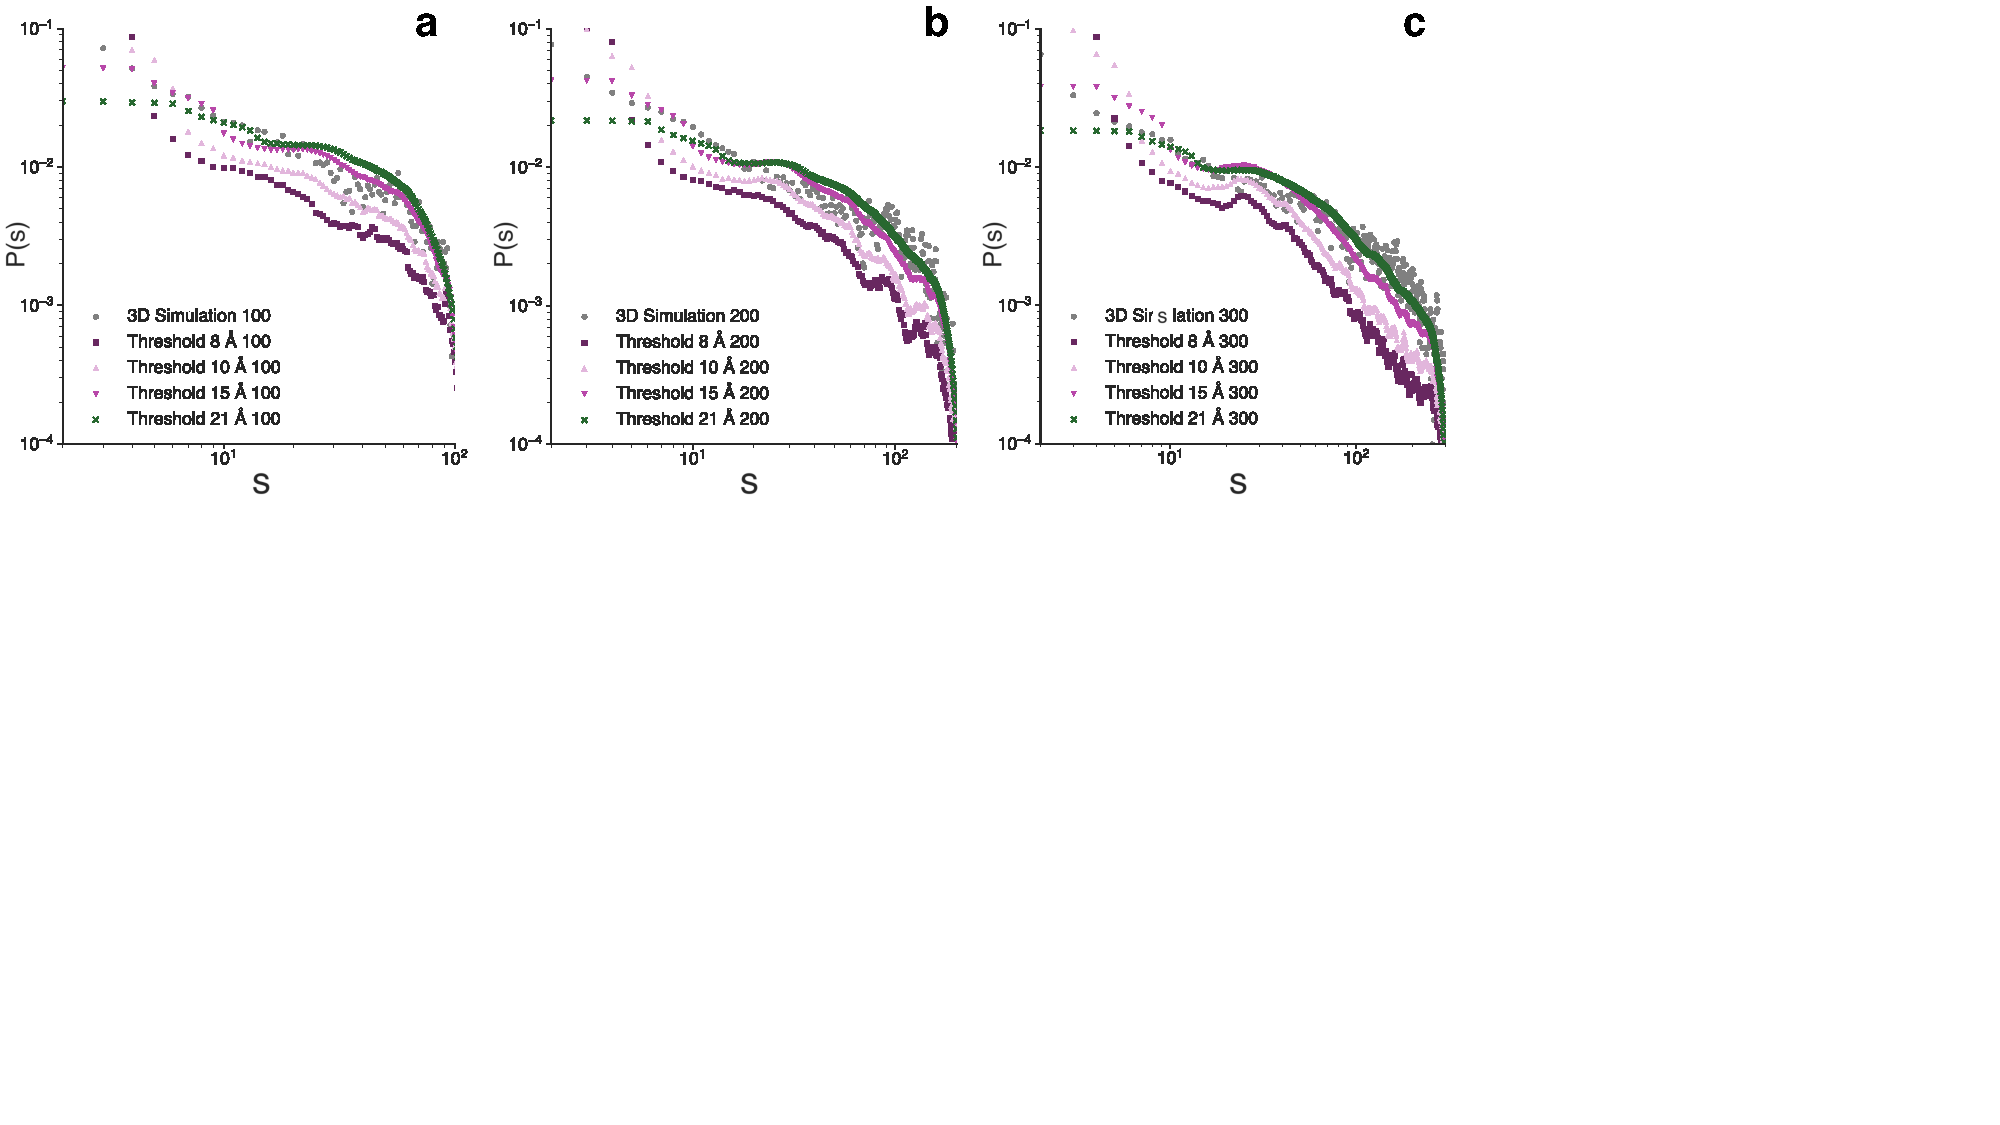
\includegraphics[width=\columnwidth]{paper/figures/SM_figures/threshold_combined.pdf}
    \caption{Amino acid distance distributions from RCSB PDB and 3D simulations for a) $L\approx100$, b) $L\approx200$ and c) $L\approx300$. Figure shows the effect of changing the threshold value $d_c$ from the default 8~Å (dark purple squares) to 10 (light purple upwards-triangles), 15 (medium purple downwards-triangles) and 21~Å (green crosses).}
    \label{fig:dc}}
\end{figure*}

\end{document}